\documentclass[12pt, letterpaper]{article}
\usepackage[margin=1in, top=0.6in]{geometry}
\usepackage{amsmath}
\usepackage{tikz}
\usepackage{titling}
\usepackage{enumitem}
\usepackage{ragged2e}
\usepackage{comment}
\usepackage{xcolor}
\usepackage[
backend=biber,
style=ieee,
sorting=none,
]{biblatex}
\addbibresource{final_bibliography.bib}
\usepackage{graphicx}
\graphicspath{{../pdf/}{figures}}
\DeclareGraphicsExtensions{.pdf,.jpeg,.png}
\usepackage{subcaption}
\usepackage{float}
\setlength{\parindent}{0pt}



\title{
    Empirical Review of Models used for Predicting Financial Market Crashes Using Market Data 
    \vspace{1em} \\
    {\large Project: Final Report}
}
\author{\normalsize Ping-Chieh Tu \\ Adrien Bélanger \\ Inigo Torres}
\date{\vspace{2em} November 22$^{\text{nd}}$ 2024}

\begin{document}

\begin{titlepage}
    \centering
    \vspace*{2in}
    {\LARGE \textbf{Empirical Review of Models used for Predicting Financial Market Crashes Using Market Data}}\\
    \vspace*{0.5in}
    {\large COMP 451 Final Project: Final Report}\\[4in]
    \normalsize
    By Ping-Chieh Tu, Adrien Bélanger, Inigo Torres \\ [3em]
    December 13$^{\text{th}}$ 2024
\end{titlepage}
\pagebreak

\subsection*{Introduction \textcolor{red}{Inigo}}

The volatility and complexity of financial markets have always been a significant challenge for the management of modern economies. 
For instance, the abrupt declines in the markets, often known in finance as crashes, can lead to widespread financial losses, economic recessions, and a loss of confidence in the stability of financial systems. 

The idea of being able to anticipate and predict such market fluctuations is not new and has been widely studied from a mathematical point of view. 
However, conventional methods used by econometricians for time series analysis, such as Linear Trend Projection or Weighted Moving Average, may be effective for markets with general stationary trends but lack effectiveness for highly volatile ones. 
Modern machine learning techniques, particularly those involving neural networks and attention-based architectures, may provide a new pathway to surpassing these traditional techniques.

In this project, we propose to make an extensive comparative study of the effectiveness of 3 of the most widely used methods for Time series forecasting today: Recurrent Neural Networks (RNNs), Transformer-based architectures, and the Autoregressive Integrated Moving Average (ARIMA) model. 

Each of these models is developed with a distinct methodological perspective. 
ARIMA models, based on classic statistics and linear algebra concepts, have long been a go-to tool for time series forecasting. 
RNNs, specifically Long Short-Term Memory (LSTM) networks, offer a non-linear and data-driven alternative that can capture long-range dependencies while reducing issues of vanishing or exploiting gradients. 
Transformers, which introduce attention mechanisms, aim to further improve predictive capabilities by focusing selectively on critical segments of past information, often achieving state-of-the-art performance in various sequential prediction tasks.

Our main objective is then to develop each of these models and subject them to a series of tests using real historical financial data to determine their effectiveness in predicting financial crashes. 

Although the world of finance is changing, and there are no specific parameters since each financial market is governed by its own rules, we will test each of these models under the same conditions and thus establish an empirical review to provide clear insights into the strengths and limitations of each methodology. We aim to guide researchers and practitioners in selecting suitable models for short-term market crash prediction, ultimately contributing to more robust risk management strategies.



\subsection*{Litterature Review \textcolor{cyan}{Adrien}}
% (Where does our project fit in context of  other articles)
    We are not the first to attempt to compare ML models performance on their prediction of market crashes using SP500 historical data. 
    Multiple approaches have been tried and tested. Time series analysis has used ARIMA and RNN based models, with the more recent addition of Transformers boosting and improving their performance  \cite{Okpeke, Ahmed, ArunKumar}. 
    Reviews of these models have been done before, but the comparison of these three models on short-term prediction using very recent market data is lacking in litterature. 
    
    \ 
    % COMPAre OTHER ARTICLES that did this

    One article compared Linear Regression and Autoregressive Moving Average (ARIMA) to predict the volatility and trend of SP500. \cite{sp500arimalstmregression}. 
    Key-findings show that ARIMA struggled on short term predictions, particularly during the 1930s and 2020 volatile markets. 
    
    Zhou et al. demonstrated that transformers handle long-term dependencies well with the "Informer model," which efficiently handles long sequences and improves trend forecasting accuracy using a "self-attention" mechanism \cite{zhou2021informer}. Moreover, Lim et al. were even able to outperform traditional methods (like ARIMA) by combining the Transformer architecture with recurrent layers \cite{lim2021temporal}. 
    
    Zhen Zeng studied the applicability of Transformers combined with RNNs in trend detection specifically for financial time series in his paper \cite{zeng2023financial}. He concluded that combining these two architectures significantly improved forecasting accuracy for intraday stock price movements of the SP500.
    
    \
    % Explore definitions of market crashes and which data was used

    Market Crashes do not hold a single definition. While historical data tags specific periods as depressions and bubbles, there are no specific metrics that are universally defined. Some have defined it as a rapid decline of 20\% or more from a recent peak over a short period \cite{Fonville, Investo}. Others still have defined them as a drawdown of 99.5\% quantile \cite{99.5quantile}.
    
    \
    % Explore models implementation
    %%% RNN
    
    Time series in the stock market often exhibit complex trends and non-linear patterns. 
    Long Short-Term Memory (LSTM) Recurrent Neural Networks (RNN) are designed to learn long-term trends in sequential data, making them very good at modeling and forecasting financial market time series \cite{hochreiter1997, greff2017}.

    LSTM networks address the vanishing gradient problem encountered in standard RNNs on this type of data by introducing specialized LSTM cells. These cells incorporate gates to control flow, allowing LSTMs to forget and remember information over long sequences \cite{hochreiter1997}.

    The LSTM cell can be defined as follows \cite{hochreiter1997}:

\begin{align*} 
    i_t &= \sigma(W_i x_t + U_i h_{t-1} + b_i), \\ f_t &= \sigma(W_f x_t + U_f h_{t-1} + b_f), \\ o_t &= \sigma(W_o x_t + U_o h_{t-1} + b_o), \\ \tilde{c}t &= \tanh(W_c x_t + U_c h{t-1} + b_c), \\ c_t &= f_t \cdot c_{t-1} + i_t \cdot \tilde{c}_t, \\ h_t &= o_t \cdot \tanh(c_t), 
\end{align*}

where

\begin{enumerate}[label=-]
    \item $x_t$ is the input at time $t$, representing market data (e.g., stock price, volume),
    \item $h_{t-1}$ is the hidden state (output) of the previous time step,
    \item $i_t$, $f_t$, $o_t$ are the input gate, forget gate, and output gate
    \item $\tilde{c}_t$ is the candidate memory cell state,
    \item $c_t$ is the cell state at time $t$, capturing long-term dependencies,
    \item $W$ and $U$ are the weight matrices and b is the bias vector,
    \item $\sigma$ is the sigmoid activation function
\end{enumerate}

The \textit{forget} gate, $f_t$, determines how much of the previous cell $c_{t-1}$ is retained. The \textit{input} gate $i_t$ updates the cell with new information. The \textit{output} gate $o_t$ controls the hidden state, which is the LSTM output at time $t$ \cite{hochreiter1997}.


%%%%%%%%%%%%%%%%%%%%%%%%
    \
    
    %%% ARIMA
    Time series in the stock market are non-stationary, which means that their statistical properties (Avg, median) change over time. ARIMA models can be adapted to capture the behavior of non-stationary time-series \cite{ho2021}. A mehodology formalized by Box et Al. in 2015 to apply the ARIMA model with a moving average component \cite{box2015}.
    This makes ARIMA suitable for predicting non-stationary time series, such as financial markets, as demonstrated by M. K. Ho et al. in their paper \cite{ho2021}.
    The ARIMA model is defined mathematically as \cite{box2015}:
    {\small
    \begin{align*}
        \varphi (B) z_t = \phi (B)\nabla^d z_t = \theta_0 + \theta (B)a_t
    \end{align*}
    where
    \begin{enumerate}[label=-]
        \item $\phi(B)$ is the autoregressive part with $p$ degrees,
        \item $\theta (B)$ is the moving average part with $q$ degrees,
        \item $\nabla$ is the integrated (degree of differencing) part with $d$ degrees,
        \item and $\theta_0$ is the constant term.
    \end{enumerate}
    }

    The use of ACF (autocorrelation function) and PACF (partial ACF) will help us decide the hyperparameters $p, d, q$ for building our model \cite{hyndman2018}, and performing Grid-Search on the specific hyperparameters will help us pin point the exact best accuracy we can get.
    
    \

    %%% TRANSFORMERS
    Transformers are based on self-attention mechanisms. They are able to weigh the importance of input elements by computing \textit{attention scores}.
    While transformers were originally developed for natural language processing tasks, they have become popular for time-series forecasting due to their ability to handle long-range dependencies \cite{vaswani2017attention}.



    Unlike RNNs, Transformers process all steps at the same time, enabling parallel computation and improved efficiency for long-range dependency learning \cite{vaswani2017attention}.

The core attention scoring by scaled dotv product is defined as \cite{vaswani2017attention}:
{\small \begin{align*} \text{Attention}(Q, K, V) = \text{softmax}\left(\frac{QK^T}{\sqrt{d_k}}\right)V, \end{align*} }
where:
\begin{enumerate}[label=-] \item $Q$ (queries), $K$ (keys), and $V$ (values) are linear projections of the input data,
\item  is the dimension of the key vectors,
\item The softmax function ensures that attention scores are normalized.
\end{enumerate}

Transformers eliminate the need for recurrent connections by relying entirely on attention mechanisms. This allows them model long-range dependencies more effectively than RNNs, which sometimes struggle with sequential bottlenecks and vanishing gradients \cite{vaswani2017attention}.

While originally developed for natural language processing tasks, Transformers have been increasingly applied to time-series forecasting \cite{zeng2023financial}.
Given the volatility and complexity of financial markets, their ability to capture complex patterns makes them an ideal choice for financial market forecasting \cite{wu2020deep}.

\

% Explore analysis criteria 
    Drastic market crashes are rare. Models can achieve extremely high accuracy by simply predicting no market crash for every datapoint \cite{market_infrequent}. Other methods are thus needed to evaluate the models. Others in litterature have used many methods, such as evaluating true positives and true negatives \cite{true_positive}. Other have used mean absolute error (MAE) to assess prediction accuracy \cite{hyndman2018}. Finally, some have used runtime and resource usage for practical feasibility to assess their performance \cite{lim2021temporal}.

\subsection*{Methodology \textcolor{cyan}{Adrien for market crash and Experiment choice} \textcolor{violet}{Everyone for their assigned model}}
% (Our models and market crash definition, how they work, why we chose them, the experiments we chose and why we chose them) + HYPOTHESIS on each experiment
Note: All code can be found in the gitHub repository linked in the Appendix.
\subsubsection*{Definitions and Metrics used in our project}

For our project, we use an LSTM-based RNN, Transformers and ARIMA to predict whether there will be a crash in the next x days based on the past y days. We defined crash as a 99.5\% quantile drawdown within a day. This gave us around 26 crashes in the test data.

To evaluate our models, we will measure the number of Predicted crashes against the real number of crashes. We will also check the number of false alarms and missed crashes. Finally, we will evaluate the training and resource usage time of all three models for each experiment.

\subsubsection*{Database and preprocessing}

We pulled the code from the SP500 public data available on Yahoo Finance financial data library. From there, we preprocessed the code by labelling crashes in the database.

Our code made use of a sliding window for the sequence length. Then, we created batches of datapoints of size 20. We then tried to predict if there would be a crash in the following shift days, which was a hyperparameter. For example, we could have a 15 day sliding window to predict if there would be a crash in the 3 days after those 15 days. 
This made the problem one of binary classification, which was simple and efficient to process, and made for easy comparison.

\subsubsection*{RNN Implementation}

Our RNN code was based on the \textit{Keras} Sequential model, using the pre-made LSTM layers \cite{keras2024lstm,keras2024sequential}. This was used since our project aimed to be a comparison, and not one of implementation. 
The code used two LSTM layers of 50 units each, then a dense layer with a sigmoid activation layer for binary classification. We then used the adam optimizer with a binary cross-entropy loss function to train our binary model.

\subsubsection*{ARIMA Implementation}
Our ARIMA code uses the default ARIMA from \textbf{statsmodels}\cite{statsmodelsARIMA} without using trend nor seasonal feature of our data. We first uses ADF test to determine the stationarity of our data. It shows that our data is non-stationary therefore the differencing term $d$ is needed. Then we looked at the PACF for decision of $p$ and ACF for decision of $q$. From PACF, we can choose either $p=0$ or $p=1$. From ACF, it is hard to tell what should be used as $q$. Therefore we run the grid search to have the hyperparameters to ensure we have a high accuracy. 

\subsubsection*{Transformers Implementation}
For our Transformer-based neural network architecture, we defined a positional encoding function (\texttt{positional\_encoding}), introducing a temporal order understanding that Transformers inherently lack. The \texttt{transformer\_model} function then constructs a model configured to accept time-series data (i.e. normalized closing prices or market indicators over a specified look-back window). Each input sequence is passed through a dense embedding layer (\texttt{Dense(embed\_dim)(x)}) and augmented with positional encodings. This enables the model to capture temporal trends more effectively. Next, a Multi-Head Attention layer selectively focuses on different parts of the input sequence, while skip connections and \texttt{LayerNormalization()} stabilize learning. The attended information is refined by a feed-forward network (Dense layers), then flattened and passed through a final sigmoid-activated layer for binary crash predictions. Finally, the model is compiled with a binary cross-entropy loss and accuracy metric to evaluate its performance on historical financial data.

\subsubsection*{Experiments}
    \begin{enumerate}
        \item 30 days sliding window, 14 days shift days\\
            Hypothesis: Here, we expect Transformers to profit from the larger sliding window, surpassing the performance of RNNs \cite{greff2017, sp500arimalstmregression}. We expect ARIMA to have the best performance of all three experiments in this one, as it has the most context and does better with more data \cite{ho2021}.
        \item 14 days sliding window, 7 days shift days
            Hypothesis: We expect that both Transformers and RNN to perform comparably by utilizing their strength in capturing medium range dependencies. Meanwhile ARIMA may also deliver reasonable results, as the window provides sufficient context for traditional statistical modeling.
        \item 7 days sliding window, 3 days shift days\\
            Hypothesis: Our belief in this experiment is that LSTM (Long Short Term Memory) based RNN models will excel due to their capability to handle shorter sequences and identify immediate dependencies effectively, as Hewamalage et al. demonstrated \cite{Hansika}: RNN architectures, and specially LSTMs can adapt well to limited sequential data, and still be able to learn patterns from it. Thus, we expect a superior performance of RNNs, followed by Transformer and ARIMA respectively.
    \end{enumerate}

    
Overall, we expect ARIMA to do good on longer sequences \cite{ho2021}. We expect RNNs to do the best with the low context of the third experiment \cite{Hansika}. Transformers should excell in higher context windows, and fall slightly behind RNNs in the third experiment. Because of the short-term nature of the experiments, we expect ARIMA to be behind the other two models in all three experiment, given the low context.
\subsection*{Empirical Evaluation \textcolor{green}{Oscar}}
% (plots, statements of comparison (without committing to a full-depth comparison, thats in discussion) of all the experiments)
From the results of the experiments, the ARIMA model has the worst performance, despite still having some correct predictions, the numerous amount of false alarms in all 3 experiments comparing to RNN and transformers which has only a few. It would be better to exclude ARIMA from the comparison and talk about it later.

\subsection*{Discussion \textcolor{violet}{Everyone discusses their experiment}}
% (discussing the results and comparing them and conclude on our hypothesis)

The results of Experiment 1, on Figure 1, present a highly skewed report. While the RNN and the Transformers performed relatively similar, with maybe slightly better overall performance on the part of the Transformers.

However, ARIMA performed very much underwhelmingly, with a prediction of over 3682 crashes. This makes 3087 false alarms, compared to 5 for RNNs and 3 for transformers. This shows that ARIMA struggled deeply with this experiment. This could be because of the way the experiment was set-up: as mentionned, ARIMA is a statistical model which needs more data to predict correctly.

While these results do go with our hypothesis, it would be unfair to say we can conclude positively on this experiment. The ARIMA model performed much under our expectation. The RNN and Transformers performed as exepcted, with Transformers having slighlt better results.

In terms of training and resource usage, the Transformers, because of their architecture, clearly beat all three with their training time and disk and RAM usage. RNN were slightly slower and consumed more disk space. ARIMA, because of our grid-search implementation, took 480 mins to compute. This is compared to the 2-3 minute training time of the other two models. ARIMA once again fell very much under our hypothesis.

In Experiment 2, RNN and Trasnformers still perform similarly. While Transformers has more correct prediction and also one more false alarm than RNN did. The results between RNN and Transformers go with out hypothesis. They both have a near 100\% prediction. As it was in Experiment 1, Transformers performed better in training time and memory usage.

\subsection*{Conclusion \textcolor{red}{Inigo}}
This empirical review project demonstrated that Recurrent Neural Networks (RNNs) and Transformer-based architectures consistently outperformed the ARIMA model in predicting financial crashes. Based on these results, we can affirm that RNNs and Transformers are better suited to capture the complex, non-linear relationships and long-range dependencies of financial time series, resulting in higher prediction accuracy of the crashes. In contrast, the ARIMA model, inherently based on linear assumptions, was  proved to be less effective in handling the volatile and non-linear nature of financial markets. Mathematically, a differenced series \((1-B)^d X_t\) is modelled as: \[ (1 - \varphi_1 B - \varphi_2 B^2 - \cdots - \varphi_p B^p)(1-B)^d X_t = (1 + \theta_1 B + \theta_2 B^2 + \cdots + \theta_q B^q)\varepsilon_t, \] where \(B\) is the backshift operator, \(\varphi_i\) and \(\theta_j\) are parameters, and \(\varepsilon_t\) is white noise. However, the ARIMA model, restricted by its linearity, assumed that the time series $X_t$ could be expressed as a linear function of its past values and past error terms and could not properly capture the sudden chaotic shifts and non-linear patterns of our financial data. Consequently, ARIMA’s linear structure leads to a less effective approximation compared to models better designed to handle non-linear patterns like RNNs or Transformers.



\subsection*{Future Directions \textcolor{red}{Inigo}}
While the superiority of Transformers and RNNs over ARIMA in predicting financial crashes is more than evident, ARIMA models could still be useful as a baseline, particularly in periods of relative market stability where linear dynamics are more pronounced. A potential avenue of improvement for this project could be to investigate the combination of RNNs/Transformers with ARIMA. For instance, during less turbulent intervals, the linear patterns captured by ARIMA can complement the non-linear adaptability of RNNs and Transformers. The linear and more conservative trend-following nature of ARIMA may be used to balance the overreaction of non-linear methods to short-term noise, decreasing false crash alarms. By intelligently combining these models, we could leverage ARIMA’s strengths for stable trend-like segments of the data while allowing more sophisticated architectures to handle the abrupt non-linear fluctuations. Regarding a more general improvement of the predictive power of our models, incorporating more macroeconomic indicators specific to each financial market and studying alternative data preprocessing techniques, such as feature engineering or advanced normalization schemes, may potentially lead to better results.



\subsection*{Self-Assessment \textcolor{green}{Oscar}}
% (how we feel about the project, what would we have done differently etc.)
From the result of this project, the RNN and Transformer models produced promising results, demonstrating their capability to capture complex temporal dependencies and effectively model market patterns leading to crashes. Howere, due to the lack of knowledge in data science, the performance of the ARIMA model fell short of expectations. With more knowledge on the fundamental of data science of preparing data and statistics, we can possibly transform the data to better fit the ARIMA model with different techniques and get better results.

\pagebreak
\subsection*{Contributions \textcolor{violet}{Everyone writes their own contribution}}
% contributions: contributions of each member to the report. If there is a disagreement, you can inlcude a longer contribution section in the appendix where each member explains their version.
\begin{enumerate}
    \item Adrien - 
        For the report, my main contributions were for writing the Litterature Review and parts of the Methodology, Discussion and Conclusion. I've also contributed to the code by implementing the RNN model, consolidating the three models in a notebook and helping design the experiments.
    \item Ping-Chieh - 
        For the report, I mainly contribute on the empirical evaluations and the self-assessment. Also provide some suggestion on the conclusion of the report. I've also make contribution to the code of ARIMA models.
    \item Inigo
\end{enumerate}


\subsection*{Appendix}
\begin{enumerate}
    \item Link to the gitHub repository with the code: \url{https://github.com/AdrienBelanger/451-Project}
    \item Figure 1: Experiment 1 Result plots 
    \begin{figure}[H]
        \centering
        \begin{subfigure}[b]{0.9\textwidth}
            \centering
            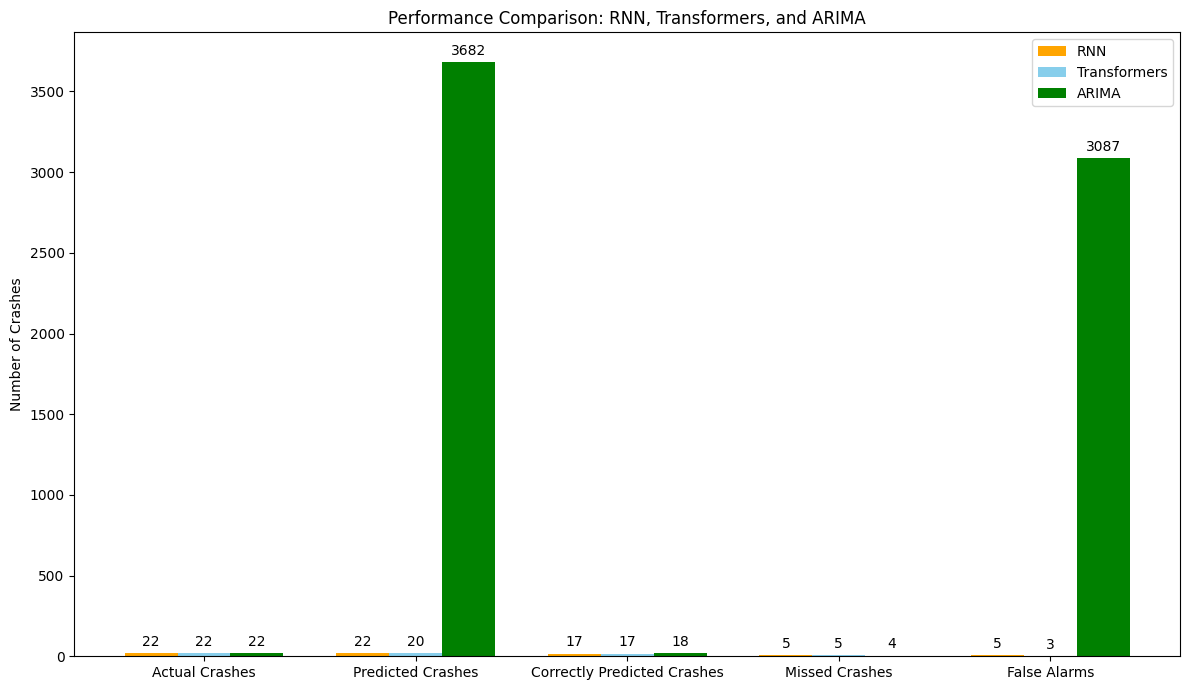
\includegraphics[width=\textwidth]{exp1_figure.png}
            \caption{Figure 1: Experiment 1 Comparison Plot}
        \end{subfigure}
        \hfill
    \end{figure}

    \item Figure 2: Experiment 2 Result plots 
    \begin{figure}[H]
        \centering
        \begin{subfigure}[b]{0.9\textwidth}
            \centering
            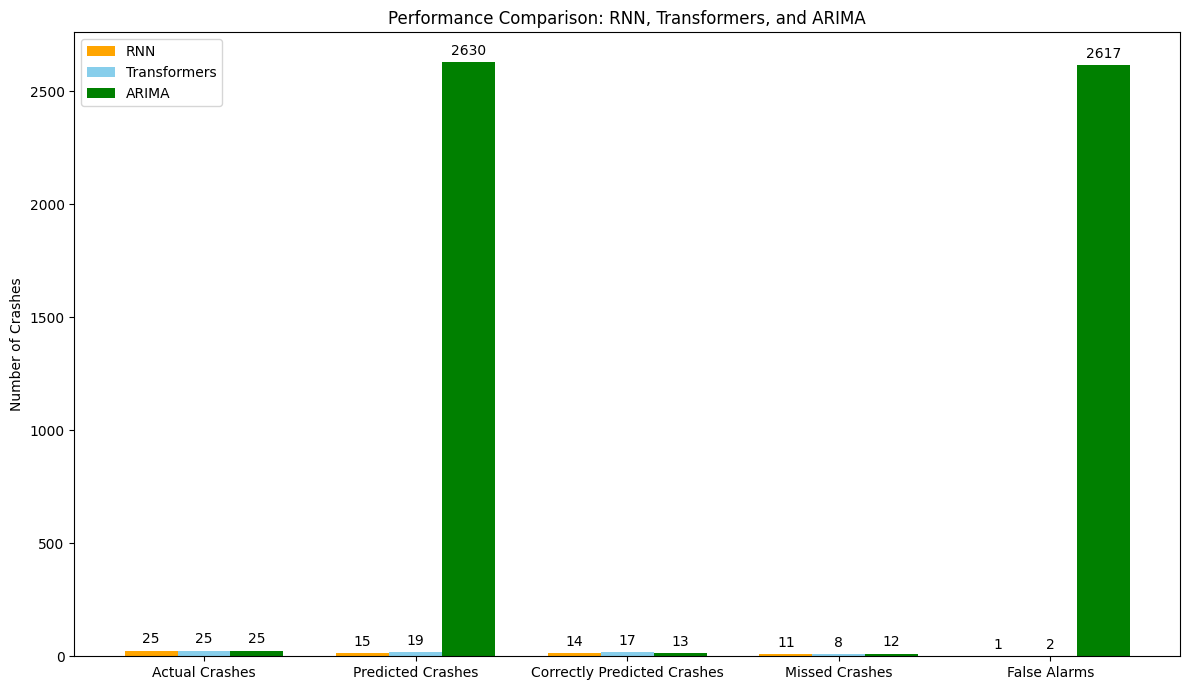
\includegraphics[width=\textwidth]{exp2_figure.png}
            \caption{Figure 2: Experiment 2 Comparison Plot}
        \end{subfigure}
        \hfill
    \end{figure}

    \item Figure 3: Experiment 3 Result plots 
    \begin{figure}[H]
        \centering
        \begin{subfigure}[b]{0.9\textwidth}
            \centering
            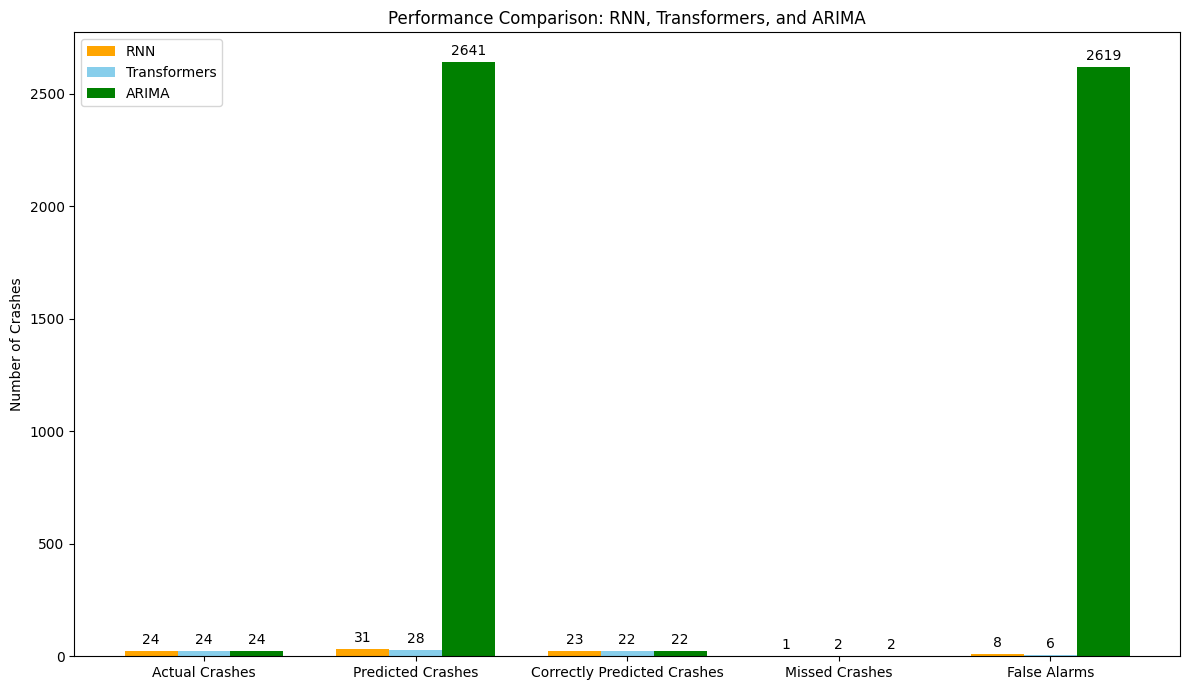
\includegraphics[width=\textwidth]{exp3_figure.png}
            \caption{Figure 3: Experiment 3 Comparison Plot}
        \end{subfigure}
        \hfill
    \end{figure}
\end{enumerate}

\printbibliography
\end{document}
